\documentclass[a4paper,11pt,dvipdfmx]{ujarticle}
% パッケージ
\usepackage{graphicx}
\usepackage{url}
% レイアウト指定を記述したファイルの読み込み
\input{layout}

% タイトルと氏名を変更せよ.
\title{日本におけるデジタル化の状況}
\author{G584922025望月 遥斗}


\begin{document}

\maketitle %ここにタイトルが入る

% ここから本文
 \section{デジタル競争力ランキング}

 国際経営開発研究所(IMD)の調査\cite{imd}によると,日本のデジタル競争力のランキングは図\ref{fig:競争力}に示すように
 調査対象の64カ国中,総合で28位,技術分野で30位となっている.
% 本文(1)
%  参考文献の参照: \cite{}
%  図番号の参照: \ref{}
% を使う
% 文献データベースのキーワードは oecd と imd
% になっている.

% 図の挿入
% を
 \begin{figure}[htbp]
    \centering
    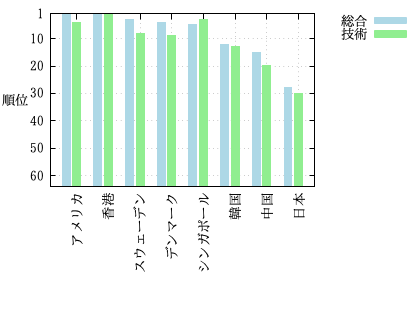
\includegraphics[width=0.7\linewidth]{fig41.png}
    \caption{デジタル競争力ランキング(64カ国中)}\label{fig:競争力}
\end{figure}
% で囲み
% \caption{}
% で図のタイトルを入れる.
% \label{}
% を使って図番号が参照できるようにする
% また,
% \centering
% で図が中央に来るようにする



\newpage
% ーーー
% 節見出し(2)
\section{ブロードバンドの整備状況}

% 本文(2)
OECDによるブロードバンド回線の普及に関する調査\cite{oecd}によると,表\ref{tbl:整備状況}に示すように,日本における 100人あたりの光ファイバー回線の加入者数は29.0で,韓国,ノルウェー,スウェーデンに続いて第4位である.

 \begin{table}[htbp]
\centering
    \caption{光ファイバー回線の加入者数(100人あたり)}
    \label{tbl:整備状況}
% 表の挿入
 \begin{tabular}{|c|l|r|}\hline
順位 & 国名 & 加入者数(\%) \\
        \hline
        1位 & 韓国 & 38.2 \\
        \hline
        2位 & スウェーデン & 31.9 \\
        \hline
        3位 & ノルウェー & 29.5 \\
        \hline
        4位 & 日本 & 29.0 \\
        \hline
        5位 & アイスランド & 28.8 \\
        \hline
        6位 & スペイン & 27.3 \\
        \hline 
        7位 & ポルトガル & 25.1 \\
        \hline
        8位 & ニュージーランド & 23.6 \\
        \hline
        9位 & リトアニア & 23.3 \\
        \hline
        10位 & フランス & 21.2 \\
        \hline
 \end{tabular}   
 \end{table} 
% による表の記述を 

% で囲み
% \caption{}
% で表のタイトルを入れる.
% \label{}
% を使って表番号が参照できるようにする
% また,
% \centering
% で表が中央に来るようにする

% ーーー
% 見出し(3)
% 考察
%  
\section{考察}

\begin{itemize}
    \item  加入者のパーセントの差が1位と2位だけ大きい
    \item  日本技術力高そうなのに総合28位、技術分野30位と思ったより低い
    \item  日本はデジタル競争力が低いのに光ファイバー加入者が多いことから人材とかほかの理由がありそう
    \item  デンマークも競争力が高いが光ファイバー加入率が低い
\end{itemize}
このことから国々の競争力と光ファイバー加入率は比例関係がないことが分かった。デジタル競争力を上げるために必要なのは光ファイバーではなく、資源の多さや、人材の多さが絡んでくると思う。
% を使って箇条書きで記述する

% ここに参考文献が入る

\bibliographystyle{junsrt}
\bibliography{exercise.bib}

\end{document}